%!TEX root=../mythesis.tex
% Chapter Template

\chapter{Late Interaction} % Main chapter title
\chaptermark{Late Interaction}  % replace the chapter name with its abbreviated form
\label{ch:late_interaction}


\section{Method}
\label{ch:late_interaction_method}
%
In this chapter, we present our next contribution designed specifically to tackle the long-standing decomposability gap problem described in~\sref{sec:open_book}.
%
Recall that in the original DPR architecture, the question $q$ and passage $p$ are encoded \emph{independently} at run time (see~\eqref{eq:dpr_encode}), which later gets multiplied to obtain the dot product as their similarity score.
%
By doing so, we effectively decompose the task of reading both $q$ and $p$ together to the task of extracting important information from each $q$ and $p$ to embedding vectors and later comparing them.
%
Our goal is to minimize the information loss caused by the extraction step.


\begin{figure}[!htbp]
	\centering
	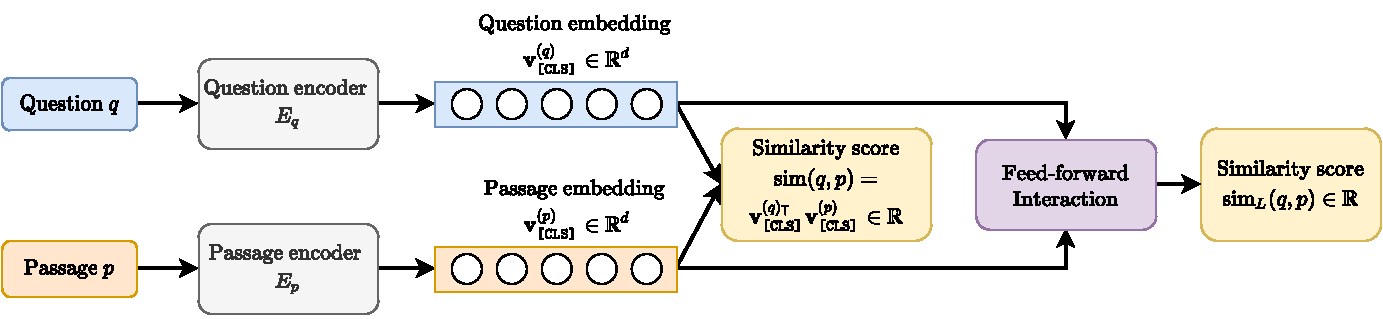
\includegraphics[width=1.0\linewidth]{late_interaction/two_tower_late_interaction.pdf}
	\caption[Two-tower architecture of DPR retriever with the late interaction mechanism.]{
		%
		The two-tower architecture of the DPR retriever with the late interaction mechanism.
		%
		After the top-$n$ retrieval with the usual similarity scores $\text{sim}(q, p)$, where $n > k$, embedding vectors are fed to the feed-forward interaction layer to obtain the late interaction similarity scores $\text{sim}_L(q, p)$, after which the final set of ranked passages is returned.
	}
	\label{fig:two_tower}
\end{figure}


%
In this work, we propose to append a small parametric module after the information extraction step.
%
This component is designed to \emph{recover} necessary information from both the question and passage embeddings that will then be compared again for retrieval, thus called \emph{late interaction}.
%
\fref{fig:two_tower} presents an overview of our proposed method.
%
Specifically, suppose we have a question embedding vector $\mathbf{v}^{(q)}_{\texttt{[CLS]}} \in \mathbb{R}^d$ and a passage embedding vector $\mathbf{v}^{(p)}_{\texttt{[CLS]}} \in \mathbb{R}^d$ obtained from the question encoder and passage encoder, respectively, using~\eqref{eq:dpr_encode}.
%
We then allows simple interactions between the two vectors
%
\begin{equation}
\label{eq:late_concat}
\mathbf{v}^{(qp)}_{\texttt{[CLS]}} = [\mathbf{v}^{(q)}_{\texttt{[CLS]}}; \mathbf{v}^{(p)}_{\texttt{[CLS]}}; \mathbf{v}^{(q)}_{\texttt{[CLS]}} \odot \mathbf{v}^{(p)}_{\texttt{[CLS]}}; \mathbf{v}^{(q)}_{\texttt{[CLS]}} - \mathbf{v}^{(p)}_{\texttt{[CLS]}}] \in \mathbb{R}^{4d}
\end{equation}
where $[\cdot;\cdot]$ denotes vector concatenation and $\odot$ denotes the Hadamard product, which is a element-wise operation.
%
We obtain $\mathbf{v}^{(qp)}_{\texttt{[CLS]}}$, a vector containing information when the question representation is allowed to interact with the passage representation on the feature level via element-wise arithmetic operations.
%
This information-rich vector is then fed through a simple feed-forward (FFN) parametric module to obtain the final similarity score
\begin{equation}
\label{eq:late_sim}
\text{sim}_L(q, p) = \mathbf{m}_L^\intercal \mathbf{v}^{(qp)}_{\texttt{[CLS]}}  \in \mathbb{R}
\end{equation}
%
where $\mathbf{m}_L \in \mathbb{R}^{4d}$ is the weight vector of the FFN.

During training, we apply the same negative log-likehood objective function defined in Definition~\ref{def:nll} to the novel late interaction similarity scores
%
\begin{equation}
L_L(q_i, p^{+}_i, p^{-}_{i, 1}, p^{-}_{i, 2}, \ldots, p^{-}_{i, n}) = - \log \frac{e^{\text{sim}_L(q_i, p^{+}_i)}}{e^{\text{sim}_L(q_i, p^{+}_i)} + \sum_{j = 1}^{n} e^{\text{sim}_L(q_i, p^{-}_{i, j})}}
\end{equation}
%
The final objective function is then taken as sum of the two individual losses
\begin{equation}
L_{\text{late\_interaction}} = L(q_i, p^{+}_i, p^{-}_{i, 1}, p^{-}_{i, 2}, \ldots, p^{-}_{i, n}) + \lambda L_L(q_i, p^{+}_i, p^{-}_{i, 1}, p^{-}_{i, 2}, \ldots, p^{-}_{i, n})
\end{equation}
%
where $\lambda$ is the weight of the late interaction objective component.
%
In other words, we train the retriever model to minimize the losses with respect to both the usual similarity scores and late-interaction similarity scores, which can also be viewed as a multi-task training paradigm.

%
At test time, we use $\text{sim}(q, p)$ for our retrieval method and $\text{sim}_L(q, p)$ for our re-ranking method.
%
In particular, given at input query $q$, we first retrieve a set $\mathcal{C_F}\prime$ of top-$n$ highest-scoring passages from a pre-built FAISS index as described in~\sref{sec:dpr_training}, where $n > k$.
%
This means that we retrieve more passages than we need.
%
Afterwards, we feed the question feature embeddings $\mathbf{v}^{(q)}_{\texttt{[CLS]}}$ as well as the embeddings of each passage in $\mathcal{C_F}\prime$ to the late interaction module via~\eqref{eq:late_concat} and~\eqref{eq:late_sim} to obtain the late-interaction similarity scores with minimal additional computational cost.
%
These scores are then used to re-rank and filter the passages in $\mathcal{C_F}\prime$ to obtain the final set $\mathcal{C_F}$ of $k$ most relevant passages.


\section{Experimental Results}
\label{ch:late_interaction_results}


\begin{table*}[t!]
	\setlength\tabcolsep{5pt}
	\centering
	\small
	\begin{tabular}{ll|cccc}
		\toprule
		\textbf{Architecture} & \textbf{Loss function}
		& Top-1 & Top-5 & Top-20 & Top-100 \\ 
		\midrule
		\multirow{2}{*}{\shortstack{DPR \\(shared encoders)}} &
		DPR loss & \textbf{53.02} & \textbf{71.30} & \textbf{80.89} & \textbf{86.93} \\
		& DPR loss + late interaction loss & 51.66 & 69.42 & 79.64 & 86.15 \\
		\bottomrule
	\end{tabular}
	\caption[Top-$\{1, 5, 20, 100\}$ retrieval accuracy on the Natural Questions test set of the DPR retriever (shared encoders) with and without the late interaction module.]{
		%
		Top-$\{1, 5, 20, 100\}$ retrieval accuracy on the Natural Questions test set of the DPR retriever (shared encoders) with and without the late interaction module, calculated as the percentage of top-$k$ retrieved passages that contain the answer.
		%
		The proposed interaction component degrades the baseline DPR model performance by a sizable margin.
	}
	
	\label{tab:shared_encoders_results}
\end{table*}


%
We conduct an experiment on NQ following the experimental settings described in~\sref{sec:exp_setup} with a batch size of 24.
%
The baseline model is taken as the DPR retriever with parameter sharing introduced in~\cref{ch:shared_encoders}, and the hyperparameters are set to $\{n, \lambda\} = \{200, 1.0\}$.
%
\tref{tab:shared_encoders_results} presents the retrieval recall on the NQ test set.

%
We observe that the late interaction component brings about a marginal performance loss to the DPR retriever.
%
We believe there are several reasons that make designing a late interaction layer difficult.
%
First, the proposed interaction layer consists of a small parametric module with weights $\mathbf{m}_L \in \mathbb{R}^{4d}$, which might not be sufficient to fully capture such complex natural language interactions.
%
Second, our interaction layer makes use of only element-wise operations (\eqref{eq:late_concat}), therefore is incapable of modeling the complex cross-feature interactions between the question embeddings and passage embeddings.
%
Lastly, it is worth noting that we did not specifically tune the newly introduced hyperparameters $\{n, \lambda\}$ which can have a huge impact on the final model performance.
%
Nevertheless, a concurrent work of~\citet{khattab2020colbert} that shares a very similar idea to our proposed late interaction has shown that this mechanism is a valuable addon to the existing retriever to combat the problem of decomposability gap.
%
Therefore, we refer interested readers to~\cite{khattab2020colbert} for a complete work on this idea.
